The following sections describe preliminary experiments conducted to assess the feasibility of the proposed vision framework.
The experiments' main focus is on the first stage \emph{S1}, as it is the foundation to develop the second stage \emph{S2}. Furthermore, there exists no work about implementing stage \emph{S1}, in opposite to self-organizing projection fibres, which are the central element of \emph{S2}.
However, to demonstrate the effectiveness of incorporating feedback from the second into the first stage, a simple mockup is used to simulate \emph{S2}.

In the following, a simple dataset is introduced in \secref{exp_dataset}. Next, the implementation of the sensory system is presented in \secref{exp_s0}, the feature extracting stage in \secref{exp_s1}, and the global feature stage in \secref{exp_s2}. he results obtained from these experiments are presented in the following \chref{results}.


\section{Dataset}\seclbl{exp_dataset}
The objective of the experiments conducted in this chapter is to demonstrate that building net fragments can be implemented using Hebbian learning \sidecite{hebb_organization_1949} (c.f. \secref{hebbian}).
Thereby, the focus is on researching novel principles as well as comprehending and analysing the networks' output rather than scaling the model to large datasets or pushing benchmarks.
Consequently, a straightforward dataset is introduced that comprises straight lines only.
Straight lines are particularly suitable for interpreting and evaluating the network's results since it is known how proper lateral support should look like (i.e. cells along a straight line should support each other).


\begin{figure}[h]
    \centering
    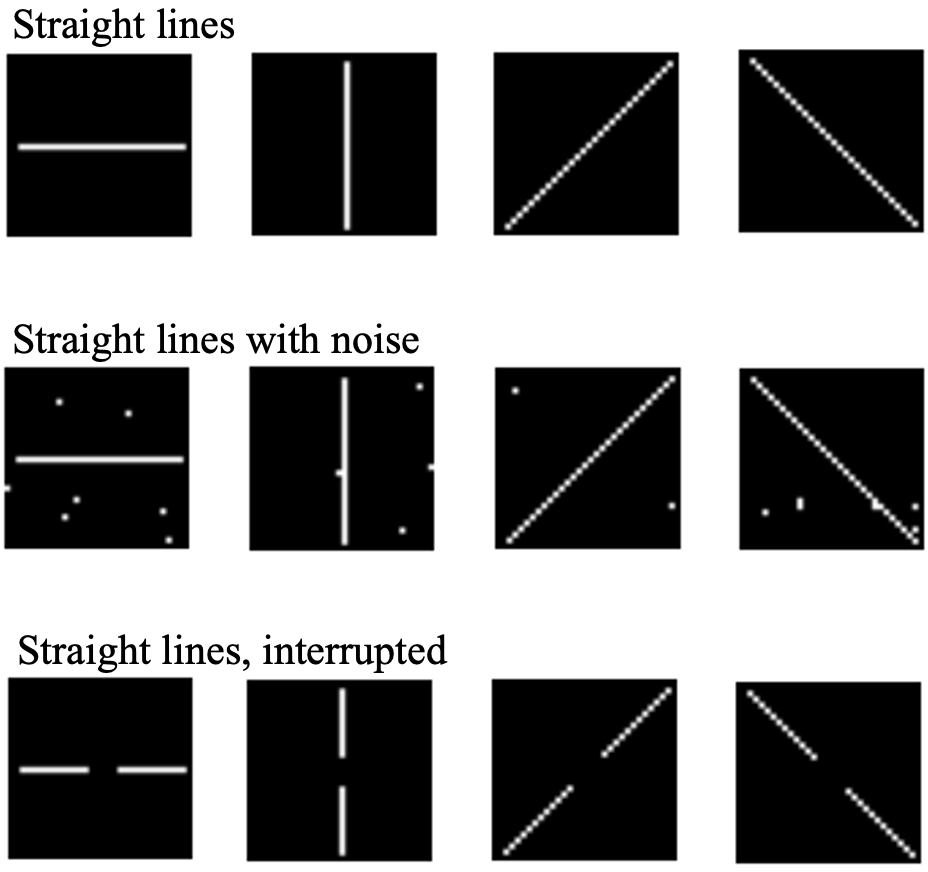
\includegraphics[width=0.59\textwidth]{straight_line_samples}
    \caption[Sample images from the dataset]{Sample images from the straight line dataset. The first row shows the images used for training, the second row the images with noise, and the third row the discontinuous lines. The images in the second and third rows are only used for evaluation.}
    \figlbl{straight_line_samples}
\end{figure}


The dataset is generated in an online fashion, meaning that images are created dynamically when required and are not stored on the disk. This provides high flexibility and allows to generate different kinds of images, especially during evaluation.
For the conducted experiments, black and white images with a dimensionality of $1 \times 32 \times 32$ are used, whereby $1$ is the number of colour channels and $32 \times 32$ is the width and the height of the image, respectively.


During \emph{training}, four fixed images are used, depicting vertical, horizontal, and two different kinds of diagonal lines (one with a positive slope and one with a negative slope). The starting and ending coordinates $(x, y)$ of these lines are as follows: A horizontal line from $(2, 16)$ to $(30, 16)$, a vertical line from $(16, 2)$ to $(16, 30)$, a diagonal line with positive slop from $(2, 2)$ to $(30, 30)$, and a diagonal line with negative slop from $(2, 30)$ to $(30, 2)$. These lines are shown in the first row of \figref{straight_line_samples}.

During \emph{testing}, different kinds of images are generated. 
First, an optional noise parameter is introduced. In this thesis, this parameter is set to $0.005$, letting each neuron with a probability of $0.5\%$ switch its activation from $0$ to $1$, or vice versa. Thus, on average, $5.12$ pixels in the image change their activation. Such images with noise are shown in the second row of \figref{straight_line_samples}.
Second, the continuous line is interrupted in the middle, resulting in a discontinuous line. The length of the break is randomly determined and within a range of $0$ to $5$ pixels. Lines with a break of $5$ pixels are shown in the last row of \figref{straight_line_samples}.
Third, a trajectory strategy is used to generate different views of an image, as described in \secref{model_overview}. This trajectory strategy allows to specify starting end ending coordinates and generates a set of lines encompassing all trajectories between these coordinates.
The result of such a trajectory strategy is shown in \figref{straight_line_trajectories}, where a horizontal line is converted to a diagonal line with a positive slope. Note that this strategy is only utilised during testing, as the required components to learn from different views during the training process have not yet been implemented. Therefore, this trajectory strategy generates images during evaluation that the network has not seen during training. 

\begin{figure}[h]
    \centering
    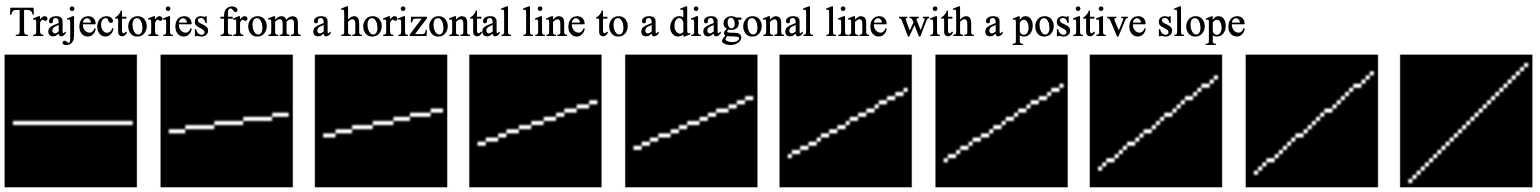
\includegraphics[width=0.99\textwidth]{straight_line_trajectories}
    \caption[Sample line trajectory strategy]{A sample trajectory strategy is applied to the horizontal line so that it becomes, over several steps, a diagonal line.}
    \figlbl{straight_line_trajectories}
\end{figure}


\section{Sensory System \emph{S0}}\seclbl{exp_s0}
The dataset used in this thesis is rather straightforward and does not require learning dedicated filters.
Furthermore, it is expected that developing a proper filter is a simple task that poses not many challenges as deep learning networks have proven themselves as excellent pattern recognition systems \sidecite{bertolini_machine_2021, bhatt_cnn_2021, zou_object_2023}.
As described in \secref{framework_s0}, the first layers of such deep networks, for example, trained in an auto-encoding setting \sidecite{rumelhart_learning_1986} with optional quantisation \sidecite{van_den_oord_neural_2017}, can be used to extract features.
It is expected that such filters would work quite well, also on natural images.
However, hand-crafted filters seem sufficient for this thesis and are preferred as they do not require additional training and can be designed to be highly interpretable. Interpretability facilitates a better understanding of the extracted features and allows a clearer comprehension of the net fragments built in the subsequent stage based on these features. 

The handcrafted filters are well-engineered, similar to what a learning system could learn.
However, they are not over-engineered. For example, it is possible to design hand-craft filters that activate one distinct channel for each line.
Such filters would simplify the task for the subsequent stages.
However, developing such filters in real-world scenarios would not be possible.
Therefore, different filters are used that create activity in all channels and ensure a realistic and representative setting.

\begin{figure}[h]
    \centering
    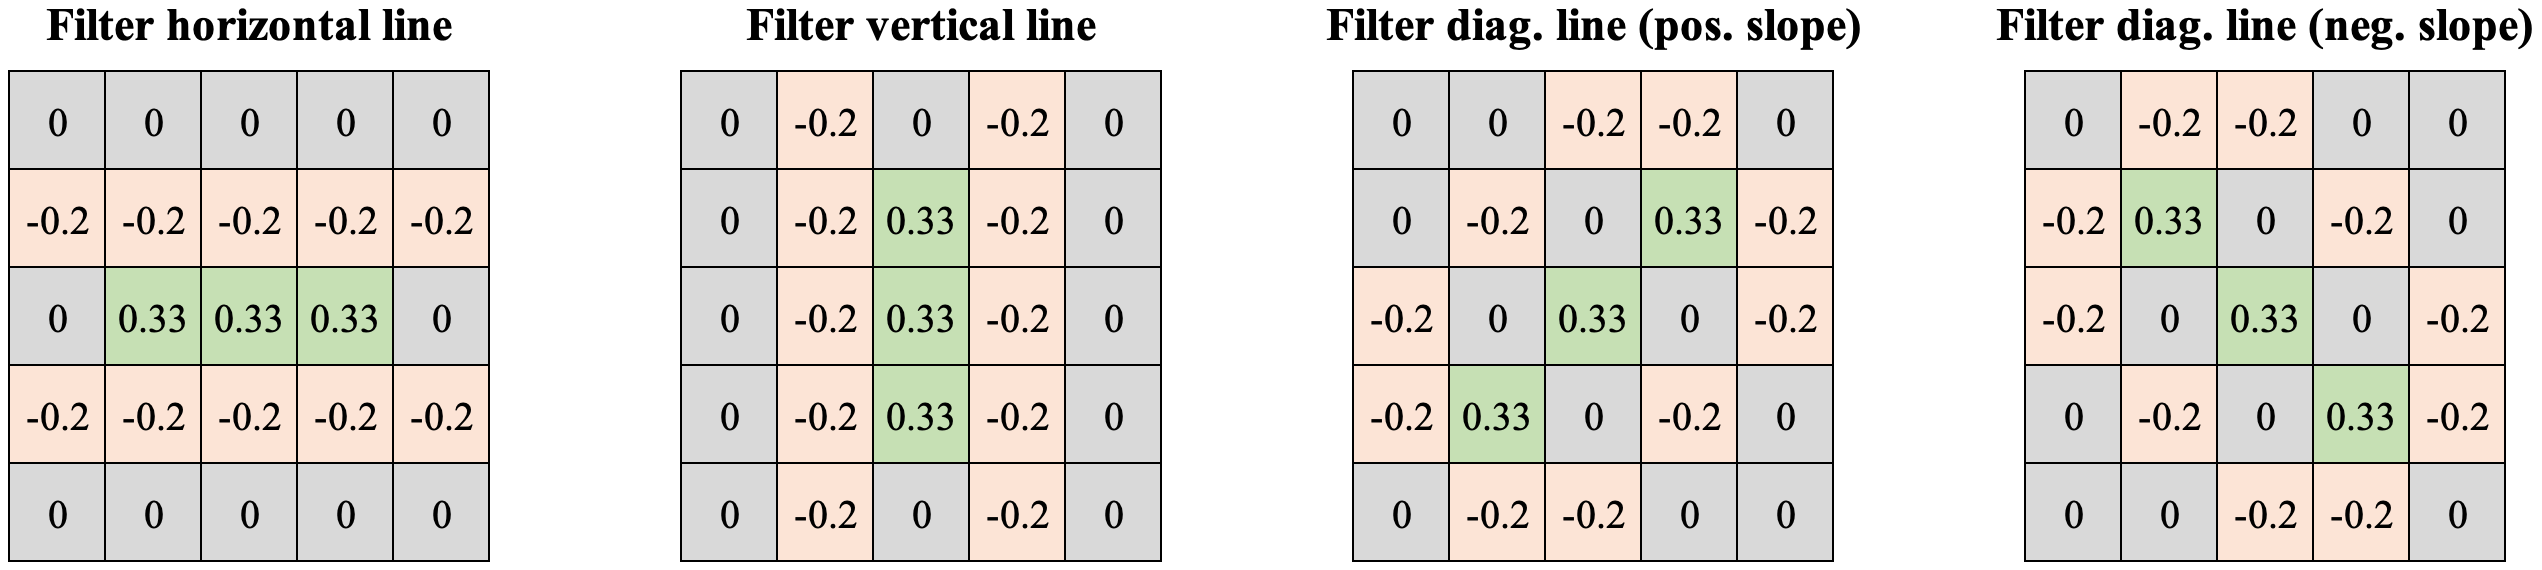
\includegraphics[width=0.99\textwidth]{filters_feature_extractor}
    \caption[Hand-crafted filters of the sensory system]{The hand-crafted filters of the sensory system that extract features from the images. The filters are optimised for horizontal, vertical, and diagonal lines.}
    \figlbl{filters_feature_extractor}
\end{figure}

The hand-crafted filters are illustrated in \figref{filters_feature_extractor}.
In total, four different filters are used, each specialising in a different type of line.
These filters function similarly to a convolutional layer with frozen (non-trainable) weights and no bias term. 
During processing, the filters are shifted with a stride of $1$ across the input image of size $(1 \times 32 \times 32)$. 
The borders are padded with $0$ values to keep the input and output sizes identical.
After applying the four filters, the output has a shape of $(4 \times 32 \times 32)$. 
However, the activations can be in a range of $-1, ..., +1$.
In order to obtain binary activations, these activations are modelled using the Bernoulli neuron.
This means that the initial activation is used as a probability value and its binary activation is sampled from a Bernoulli distribution.


\begin{figure}[h]
    \centering
    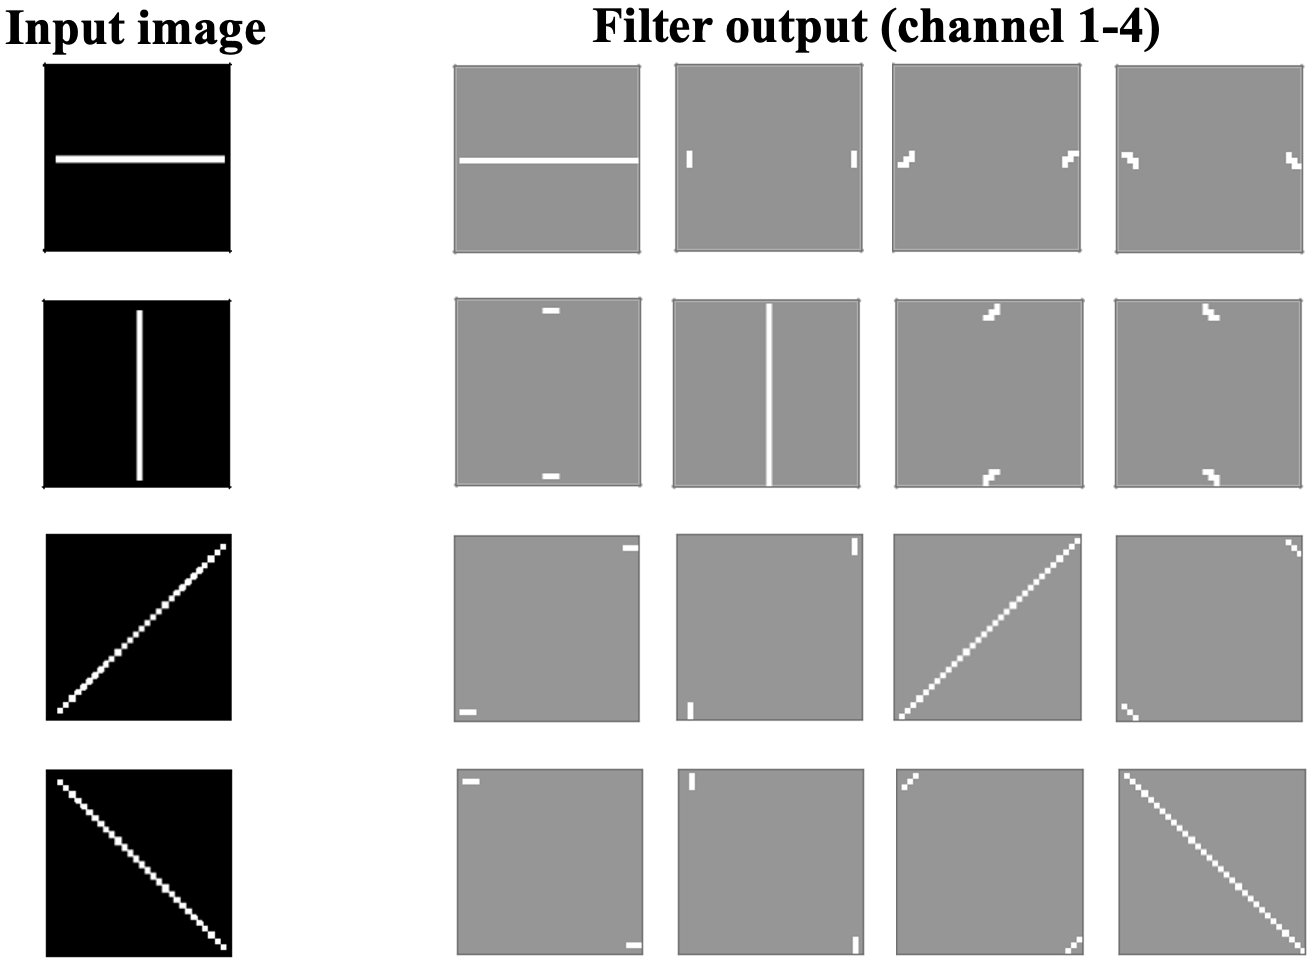
\includegraphics[width=0.99\textwidth]{results_filter}
    \caption[Output of hand-crafted filters for straight lines]{Output of hand-crafted filters for the straight lines used during training. Each row shows the input image (on the left) and the responses of the four filters (on the right).}
    \figlbl{result_filter}
\end{figure}

\figref{result_filter} shows the filter response if these four filters are applied to the images form the training dataset.
Please not that a fixed threshold of $0.5$ instead of a Bernoulli neuron is used to create this figure, so that it appears visually less noisy.
For each type of line, one filter specialising in this line has a very strong response, almost reassembling the input image (except extending the line by a few pixels).
The other filters primarily activate around the endpoints of the lines.


\section{Feature Extracting Stage \emph{S1}}\seclbl{exp_s1}
The sensory signal of shape $(4 \times 32 \times 32)$ is further processed by the feature extracting stage to build net fragments. In the conducted experiments, no alternative cells are used and therefore the output of \emph{S1} is of the same shape as the input signal, i.e. $(4 \times 32 \times 32)$.
However, as described in \secref{framework_s1}, the input of \emph{S1} consists not only of the signal from the sensory system, but also of the previous net fragments that can be overridden by the feedback from the object prototypes.
These inputs are stacked along the first dimension, resulting in an input matrix of shape $(8 \times 32 \times 32)$ and an output of shape $(4 \times 32 \times 32)$.
Thereby, the first four channels (i.e. the input with index $(1, ..., 4 \times H \times W)$) are the output of the sensory system and last four channels (i.e. input with index $(5, ..., 8 \times H \times W)$) are the previous net fragments.
The previous net fragments are overridden by the feedback of \emph{S2} if the mean square error between the net fragments and the \emph{S2} feedback is below a threshold value of $0.05$ and thus the feedback is considered credible.










The lateral support reach of a single cell is defined as $n_l=5$. Thus, a cell can get lateral supported by all cells not further away than $5$ cells in each direction, or $2n_l+1=11$ along the vertical and horizontal axis.
The lateral support could be implemented by using a convolutional kernel $\boldsymbol{W}$ of size $(4 \times 8 \times 11 \times 11)$. However, implementing this kernel in practice so that Hebbian updates can efficiently be calculates requires two kernels. This procedure is described in \secref{exp_conv_details}.



















\subsection{Support Implementation Details}\seclbl{exp_conv_details}
Implementing Hebbian updates efficiently in a deep learning framework is not trivial: In an efficient implementation, the kernel is not shifted from cell to cell. Instead, a circulant matrix is built so that all kernel updates can be calculated in parallel. However, by applying this operation, information about the cell's lateral influence is lost.

A solution to this problem is proposed by \sideciteay{miconi_hebbian_2021}. He uses a loss function whose derivative is exactly the Hebbian update. By doing so, backpropagation of error can be used to update the weights, whereby the weight update is similar to the Hebbian rule.
This allows a very efficient Hebbian training for convolutional layers.
However, this approach is quite limited and does not provide the flexibility needed to implement all parts of the proposed framework.

In this thesis, a different implementation is proposed that comes with a slight memory overhead, but is very efficient and does not rely on backpropagation at all. The proposed method is based on two convolutional layers: The first layer is a fixed, binary convolution that restructures each input patch into a single-column vector. This is followed by a $1\times1$ convolution containing the actual weights. Specifically, we can pass the input through a fixed convolution with an input size of $C_{in} \times 2n_l+1 \times 2n_l+1$ and $C_{in} 2(2n_l+1)$ output channels. The weight vector for this convolution is set to $1$ for the connections linking input $c_i,w,h$ to output $c_iwh$ (where $c_i$ $w$, and $h$ range from 1 to $C_{in}$, $2n+1$, and $2n+1$, respectively), and it is set to 0 everywhere else. This process reorganises the values of each input patch from the original convolution into non-overlapping column vectors, effectively duplicating them. Next, the actual weights of the original convolution using can be applied using a simple $1\times1$ convolution. This can be achieved by performing a tensor product with appropriate broadcasting.
Thus, the proposed method allows to calculate Hebbian updates while fully leveraging the computational capabilities of current deep learning hardware.








\section{Global Feature Stage \emph{S2}}\seclbl{exp_s2}






